\chapter{Introducción}

%Este proyecto es software libre, y está liberado con la licencia \cite{gplv3}.

A continuación se presentan los fundamentos teóricos necesarios para comprender el trabajo realizado.
%, así como el proceso de planificación y desarrollo realizado y las conclusiones y resultados obtenidos.


\section{Gestión de dispositivos astronómicos distribuidos}
% Descripción no formal del proyecto. ¿Que vamos a hacer?

Este proyecto simula un encargo profesional, en el cual, de acuerdo a las necesidades del cliente, se desarrollará \textbf{un cliente web capaz de gestionar dispositivos astronómicos de manera inalámbrica}. 

La comunidad de astronomía y astrofotografía se ayuda de una gran variedad de intrumentos de observación con el fin de estudiar los astros celestes. Los avances tecnológicos modernos permiten que \textbf{telescopios, cámaras, y toda clase de accesorios especializados} se gestionen como \textbf{dispositivos distribuidos independientes}, con una infinidad de parámetros modificables. Con el objetivo de facilitar la gestión y sincronización de estos, se han desarrollado una multitud de protocolos y librerías. Durante el desarrollo de nuestro proyecto, nos apoyaremos en estas tecnologías, investigando su funcionamiento y los diversas herramientas y librerías que ofrecen. 


%IMAGEN 
\begin{figure}[h]
	\centering
	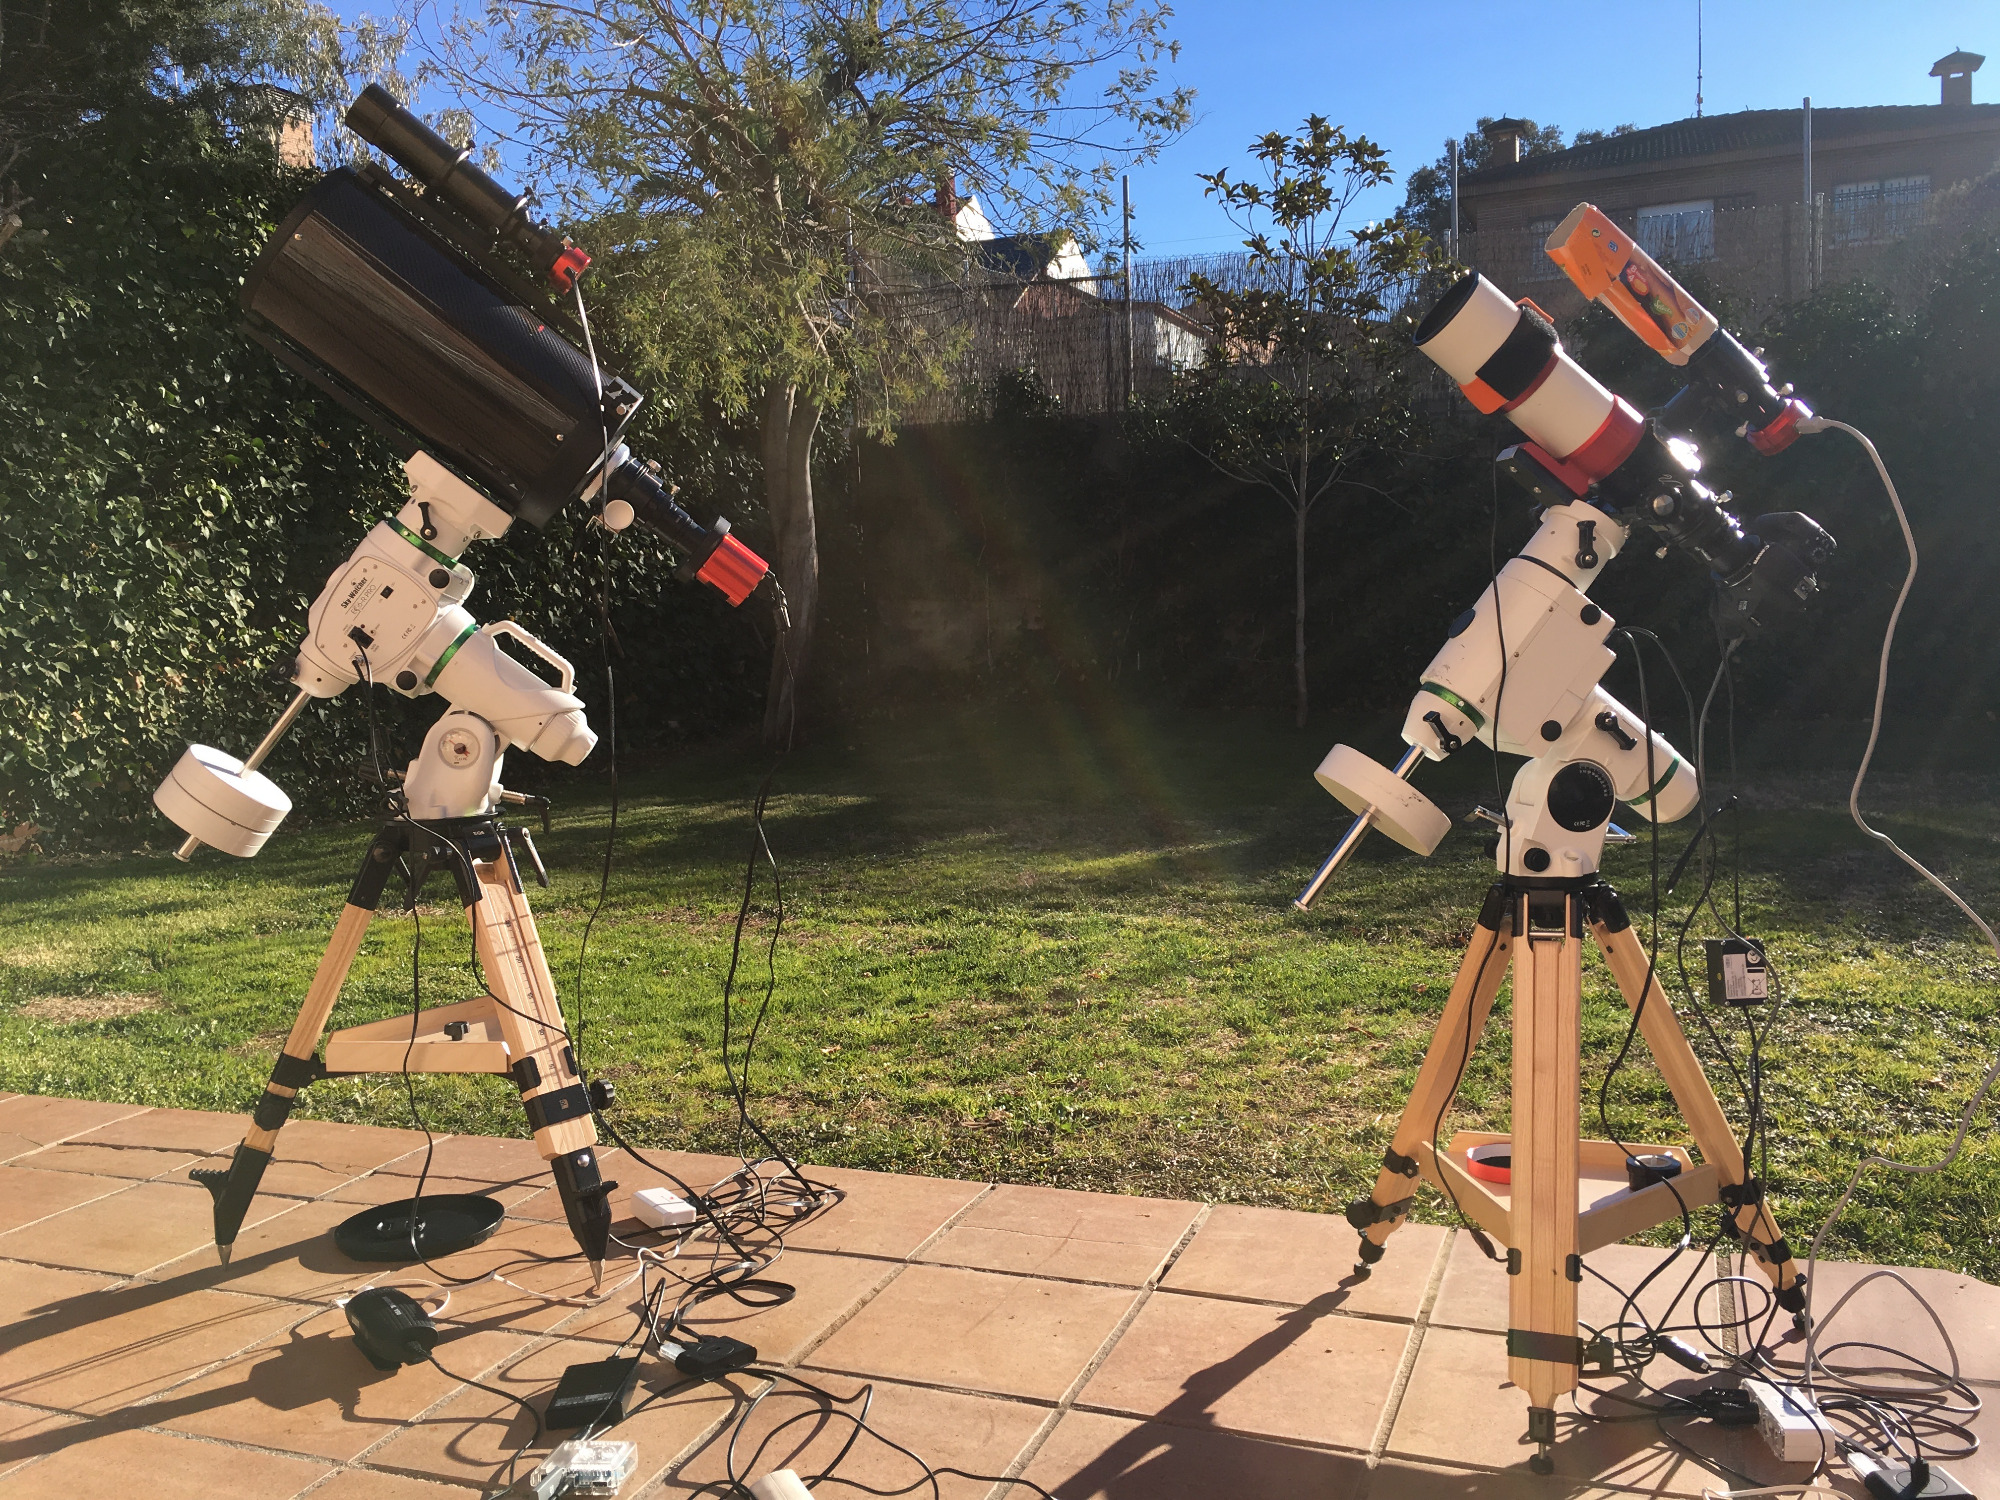
\includegraphics[scale=0.20]{img/astrophotography.jpg}
	\caption{Ejemplo de un \textit{setup} de astrofotografía, con dos telescopios con filtros, monturas y cámaras CCD.}
\end{figure}


A continuación se describen los protocolos más utilizados en el campo y las ventajas que presenta el protocolo seleccionado con respecto a otras alternativas.


\subsection{ASCOM: Astronomy Common Object Model}

\textbf{ASCOM}\cite{ascom} (abreviación de Astronomy Common Object Model) es una iniciativa de codigo abierto ampliamente adoptada en la comunidad astronómica. Creada en 1997, ASCOM fue creado en un momento en el que la falta de un protocolo estandarizado generaba problemas a la hora de integrar hardware de distintos fabricantes. ASCOM se estableció como una serie de estándares y especificaciones universales para aplicaciones (APIs), con el objetivo de eliminar la necesidad de escribir código personalizado para cada dispositivo y sus drivers por cada aplicación, ofreciendo una interfaz universal y síncrona que facilitase la interoperabilidad. 

La implementación inicial de ASCOM se conoce como \textbf{ASCOM COM}\cite{ascom-com}, en referencia a la tecnología de comunicaciones COM (Component Object Model) implementada por Microsoft. Dado que está diseñado alrededor del modelo COM, su uso está completamente limitado al entorno de trabajo de Windows y .Net, lo que limita su uso en cualquier otro sistema operativo, por lo que no cumple los requisitos para nuestro proyecto. 

Para superar esta limitación, se ha desarrollado una implementación más moderna de ASCOM, conocida como \textbf{ASCOM Alpaca}\cite{ascom-alpaca}, o simplemente \textbf{ALPACA}. Esta versión del protocolo se basa en comunicación a través de redes IP, utilizando protocolos HTTP y REST, lo que permite su funcionamiento no solo en sistemas Linux, MacOS y Windows, sino también en dispositivos astronómicos con controladores embedidos. Aunque ALPACA podría cumplir nuestras necesidades en teoría, esta implementación todavía es relativamente reciente, y depende en gran medida de la estructura y los drivers ya establecidos en ASCOM COM.

Sumado a todo esto, el protocolo establecido por ASCOM posee una estructura exclusivamente síncrona, lo que restringe significativamente nuestras posibilidades a la hora de diseñar la aplicación. Esta limitación, sumada a las anteriores mencionadas, nos lleva a concluir que ASCOM, a pesar de su amplia adopción, es una opción menos adecuada para nuestro proyecto en comparación con alternativas más flexibles como \textbf{el protocolo INDI} y su bifurcación, \textbf{el protocolo INDIGO}.


\subsection{INDI: Instrument Neutral Distributed Interface}

\textbf{El protocolo INDI}\cite{indi-library} (abreviación de Instrument Neutral Distributed Interface) es un estándar de comunicación de software libre diseñado para dispositivos astronomicos. Fue creado por Elwood Downey en 2003 con el objetivo de crear un protocolo de control en el que la comunicación fuese \textbf{independiente de la plataforma y el cliente}, inicialmente ideado como parte del desarrollo del software de planetario KStars\cite{kstars}, y actualmente adoptado y expandido por la comunidad astronómica.

Es un protocolo de comunicación \textbf{asíncrono y multiplataforma}, basado en la transmisión de mensajes XML a través de redes TCP/IP. Su arquitectura se basa en un modelo cliente-servidor, implementando un \textbf{servidor INDI} que se conecta a los dispositivos astronómicos y actua como intermediario entre estos y las aplicaciones de control a través de mensajes XML. El servidor desempeña el papel de hub central, gestionando los controladores de los dispositivos y redirigiendo la información bidireccionalmente entre dispositivo y cliente. Este enfoque libera al cliente de la carga de gestionar directamente los dispositivos, permitiéndole actuar exclusivamente como front-end y construir dinámicamente su conocimiento de los dispositivos en tiempo de ejecución. Para una explicación más profunda sobre el funcionamiento de este protocolo y su arquitectura se puede consultar el \textit{whitepaper} de INDI\cite{indi-whitepaper}.

Es extremadamente extensible, permitiendo añadir o retirar cualquier clase de dispositivo sin necesidad de rediseñar la estructura, y está diseñado para ser modular. Además, la comunicación basada en XML asegura que la información transmitida sea ligera, fácil de interpretar, y no esté limitada a ningún sistema operativo en particular.

%COMPLETAR: Un párrafo de transición a INDIGO como fork de INDI.

\subsection{INDIGO Astronomy}

\textbf{INDIGO Astronomy}\cite{indigo} es una bifurcación del protocolo INDI creada en 2016 por Peter Polakovic y otros miembros de la comunidad de INDI con el objetivo de solucionar algunas limitaciones técnicas presentes en el protocolo original. 

Aunque INDIGO es desarrollado de cero, se basa en los principios propuestos por INDI. Al igual que este, mantiene la \textbf{estructura cliente-servidor} y la \textbf{comunicación a través de redes TCP/IP} que lo caracterizan, lo que garantiza la compatibilidad, extensibilidad, y el soporte multiplataforma. Sin embargo, la principal diferencia entre ambos es su \textbf{arquitectura}. Mientras que en INDI los controladores y los clientes de manera independiente se comunican a través de una red, INDIGO introduce un bus de software dedicado para la comunicación entre estos componentes. En el mejor de los casos, esta mejora puede aumentar significativamente la velocidad de las operaciones sin comprometer la estructura distribuida. 

INDIGO garantiza una \textbf{total compatibilidad con clientes y servidores INDI}, y también implementa funciones wrappers para maximizar en el mayor grado posible \textbf{Compatibilidad con clientes y servidores ASCOM y ALPACA}. 

El framework de INDIGO ofrece una gran variedad de herramientas software que hacen uso del protocolo. La infraestructura principal de INDIGO incluye utilidades basadas en consola como \textbf{INDIGO Server}, que permite, con un solo comando, el despliegue rápido del servidor y la detección automática de dispositivos conectados a la red, y otras como \textbf{INDIGO Prop Tool}, que facilita la configuración del servidor y gestión de las propiedades de sus dispositivos. También implementa su propio cliente GUI, \textbf{INDIGO Control Panel}. Estas herramientas serán de gran utilidad durante la investigación del protocolo y el testeo de sus funcionalidades.\cite{indigo-drivers}

%IMAGEN 
\begin{figure}[h]
	\centering
	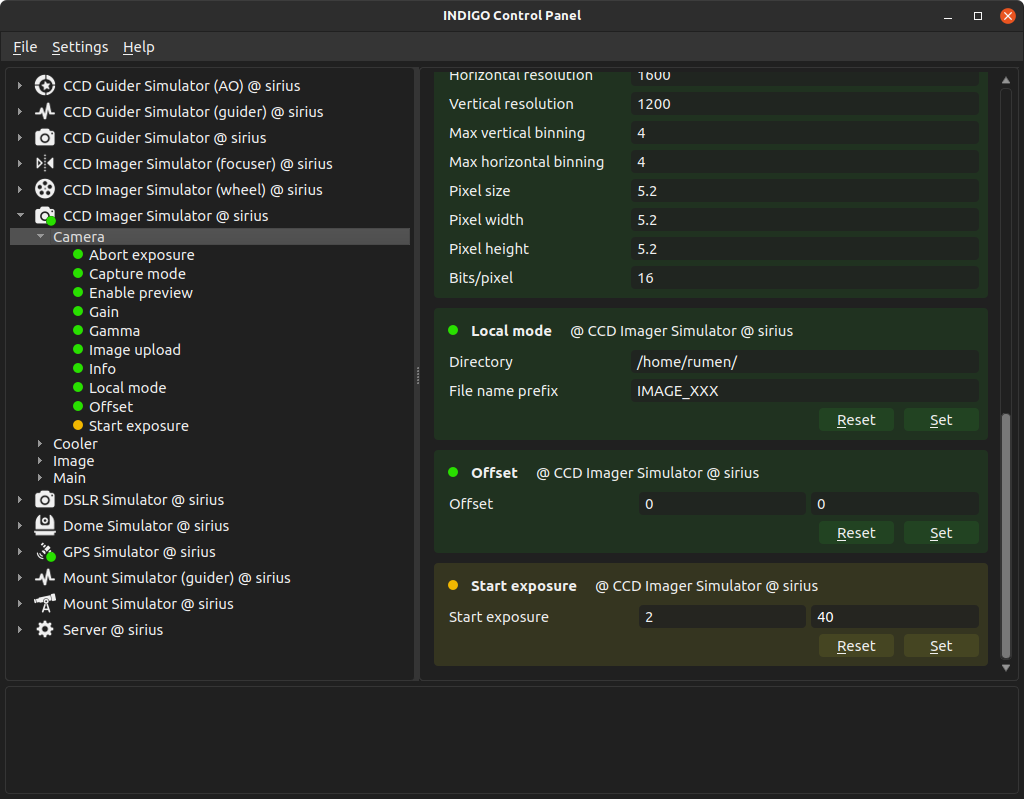
\includegraphics[scale=0.40]{img/indigo-control-panel.png}
	\caption{INDIGO Control Panel, cliente GUI para gestionar dispositivos astronómicos.}
\end{figure}


La comunidad usuarios y desarrolladores de INDIGO es particularmente activa, con frecuentes contribuciones y actualizaciones de la plataforma. INDIGO cuenta con un extenso repertorio de drivers disponibles, el cual está en constante expansión gracias al desarrollo activo y colaborativo de la comunidad en GitHub\cite{indigo-repository}. Además, disponen de un grupo de usuarios con un foro dedicado, donde se comparten conocimientos sobre el campo de la astronomía y la tecnología de INDIGO, se resuleven dudas y se ofrece apoyo técnico en cualquier momento, lo que nos podría ser de gran utilidad a la hora de familiarizarnos con esta tecnología.\cite{indigo-forum}

% EXPANDIR: Una posible falla es que en Linux y MacOS se han implementado tanto cliente como servidor pero en WIndows solo se ha implementado Cliente

\section{Crítica}

La principal desventaja de los protocolos anteriormente descritos es su dependencia en un cliente con interfaz gráfica de usuario para la gestión e interpretación de las propiedades del servidor. Si bien estos protocolos ofrecen sus propias implementaciones, el uso de estas herramientas requiere una preparación e instalación previa, lo cual no siempre es posible o conveniente en todas las máquinas. Un ejemplo claro de esto se ve en las herramientas del protocolo ASCOM, cuyo uso está principalmente restringido a sistemas operativos Windows. En una entorno ideal, el cliente sea capaz de poder funcionar independientemente de la plataforma.

Además, en un ámbito como la astronomía se valora mucho las soluciones ligeras y eficientes en su consumo de recursos, dado que la gestión simultánea de múltiples dispositivos distribuidos requiere de un uso optimizado de la memoria y CPU para poder maximizar el tiempo de uso de los dispositivos y su eficiencia durante una sesión de observación en el campo.


El protocolo INDIGO, con su infraestructura optimizada y conexión eficiente es el que mejor se ajusta a las necesidades de este tipo de proyectos. No obstante, a pesar de que su herramienta GUI está disponible en sistema operativos como Linux, MacOS y Windows, sufre del mismo problema, la necesidad de una instalación previa. Esto puede reducir su accesibilidad en dispositivos más ligeros como dispositivos móviles.

INDIGO, con su estructura de mensajes fácilmente interpretable, permite a los usuarios desarrollar sus propios clientes y herramientas a través de código para gestionar el intercambio de mensajes con el servidor, sin tener que depender del software provisto por el equipo de desarrollo. Esto permite al usuario crear soluciones personalizadas que se adapten a las necesidades específicas. Sin embargo la mayor parte de la comunidad de INDIGO se limita al uso del software que provee el protocolo, y las alternativas de código abierto disponibles son pocas y están limitadas a ciertos lenguajes de programación específicos, como Python. Por tanto, recae sobre el usuario la responsabilidad de no solo aprender el funcionamiento del protocolo, sino también adquirir los conocimientos de programación necesarios para poder crear una solución que satisfaga sus necesidades particulares.


\section{Propuesta}

Teniendo en cuenta las tecnologías a nuestra disposición y sus características y limitaciones, se propone el desarrollo de un cliente web capaz de gestionar dispositivos astronómicos haciendo uso del protocolo INDIGO, anteriormente descrito. Este cliente será diseñado a dos niveles claramente distinguidos:

\begin{itemize}
  \item \textbf{Primer nivel:} consistirá en una biblioteca en JavaScript, que actue como cliente INDIGO. Esta biblioteca se encargará de la comunicación con un servidor INDIGO, y permitirá la gestión de las propiedades de los dispositivos conectados a este.
  \item \textbf{Segundo nivel:} consistirá en una interfaz gráfica de usuario, que haciendo uso de la biblioteca JavaScript desarrollada en el primer nivel, permitirá una interpretación y gestión sencilla de las propiedades del servidor y sus dispositivos.
\end{itemize}


Para este proyecto, utilizaremos las herramientas proporcionadas por el equipo de desarrollo de la iniciativa INDIGO. Con el software INDIGO Server, tendremos acceso a un servidor INDIGO altamente configurable a través de la línea de comandos, al cual conectaremos nuestro cliente. Además, la distribución de INDIGO incluye entre su extensa lista de drivers multiples simuladores de dispositivos astronómicos, como cámaras CCD, monturas y GPS, de los que nos ayudaremos para realizar pruebas y validar el funcionamiento de nuestro cliente.

\subsection{Requisitos}

A continuación se presenta una lista de los requisitos funcionales y no funcionales inicialmente planteados para definir nuestra aplicación. Se hace distinción entre los requisitos de la biblioteca cliente, y los requisitos de la interfaz gráfica.

\subsubsection{Requisitos de la biblioteca}

\textbf{Requisitos funcionales de la biblioteca.}

\begin{enumerate}[label=\textbf{R1.1.\arabic*.}, leftmargin=10mm]
  \item La biblioteca debe ser capaz de establecer conexiones con el dispositivo/servidor INDIGO utilizando protocolos WebSocket.
  \item La biblioteca debe ser capaz de enviar mensajes y recibir mensajes del servidor en tiempo real.
  \item La biblioteca debe gestionar posibles errores de conexión y reintentar la conexión automáticamente si es necesario.
  \item La biblioteca deberá ser capaz de procesar los mensajes del protocolo INDIGO recibidos del dispositivo y generar respuestas apropiadas para estos en JSON.
  \item La biblioteca debe implementar mecanismos de detección de errores en la comunicación y el procesamiento de datos, alertando al usuario cuando se produzca un fallo.
  \item La biblioteca debe ser capaz de solicitar al dispositivo un listado de todas las Propiedades. 
  \item La biblioteca debe solicitar el listado de las Propiedades del dispositivo al iniciar la conexión 
  \item La biblioteca debe ser capaz de procesar los distintos tipos de Propiedades existentes en el protocolo INDI: text, number, switch, lights, y BLOB.
  \item La biblioteca debe almacenar en tiempo real la información recibida del Dispositivo y sus Propiedades en una estructura interna de clases.
  \item La biblioteca debe ser capaz de enviar solicitudes de modificación de una o más Propiedades conocidas previamente.
  \item La biblioteca debe gestionar los diferentes estados de las Propiedades y actuar según estos.
  \item La biblioteca debe permitir eliminar Dispositivos o Propiedades de su estructura interna si recibe una señal de borrado desde el servidor.
  \item Será posible establecer si el Dispositivo tiene o no permisos para enviar BLOBs a través del WebSocket (Never, Also, Only)
  \item La biblioteca debe ser configurable para permitir a los usuarios ajustar parámetros
\end{enumerate}


\textbf{Requisitos no funcionales de la biblioteca.}

\begin{enumerate}[label=\textbf{R1.2.\arabic*.}, leftmargin=10mm]
  \item La biblioteca debe estar optimizada para hacer su uso eficiente en cualquier clase de dispositivo.
  \item La biblioteca debe ser compatible con múltiples sistemas operativos.
  \item La biblioteca debe empaquetar todos sus componentes en un único archivo fácilmente distribuible.
  \item La biblioteca debe ser empaquetada y preparada para múltiples patrones y formatos de módulos de programación en JavaScript (CommonJS, ECMAScript Modules, IIFE...).
\end{enumerate}


\subsubsection{Requisitos de la interfaz gráfica}  

\textbf{Requisitos funcionales de la interfaz gráfica.}

\begin{enumerate}[label=\textbf{R2.1\arabic*}, leftmargin=10mm]
  \item La interfaz debe almacenar localmente una lista de los dispositivos disponibles y de cada uno de sus propiedades.
  \item La interfaz debe mostrar al usuario desde el cliente un listado de las propiedades de todos los dispositivos conectados.
  \item La interfaz debe actualizar en tiempo real las propiedades de un dispositivo en consonancia con los cambios que se realicen en el servidor.
  \item La interfaz debe permitir enviar al servidor solicitudes de modificación de uno o más elementos de una Propiedad en tiempo real.
  \item La interfaz debe limitar el acceso y modificación de las propiedades en función de su estado y permisos.
  \item La interfaz debe gestionar el estado de las propiedades registradas dentro del cliente independientemente de las respuestas del servidor.
  \item La interfaz debe eliminar propiedades o dispositivos de la lista conforme lleguen solicitudes desde los dispositivos.
  \item La interfaz debe permitir programar cambios específicos de las propiedades a horas determinadas.
\end{enumerate}



\textbf{Requisitos no funcionales de la interfaz gráfica.}

\begin{enumerate}[label=\textbf{R2.2\arabic*.}, leftmargin=10mm]
  \item La interfaz debe hacer uso de la biblioteca JavaScript anteriormente definida como cliente.
  \item La interfaz debe ser sencilla y compatible con toda clase de dispositivos.
  \item La estructura de datos de la interfaz será local y dinámicamente construida.
  
\end{enumerate}


\section{Conocimientos previos}

Para el desarrollo de este proyecto, se han puesto en práctica conocimientos adquiridos a lo largo del grado de Ingeniería informática. A continuación se detallan las asignaturas específicas que han sido fundamentales, aunque se entiende que esta no es una lista exhaustiva y que todos los conocimientos adquiridos durante el grado han contribuido al desarrollo general del proyecto.

\subsection{Conocimientos de desarrollo web}
Los conocimientos de programación en HTML y JavaScript adquiridos en las siguientes materiales han servido como base fundamental para el desarrollo de tanto la biblioteca en Javascript como la interfaz gráfica, y sus interacciones:

\begin{itemize}
	\item Fundamentos de Redes
	\item Sistemas de Información Basados en Web
	\item Sistemas Gráficos
	\item Diseño de Interfaces de Usuario
\end{itemize}


\subsection{Conocimientos de programación orientada a objetos}
Los conocimientos de programación orientada a objetos adquiridos en estas asignaturas han servido para desarrollar la aplicación cliente en Javascript junto con su estructura de datos, y la comunicación por mensajes a través de TCP/IP entre cliente y servidor. 

\begin{itemize}
	\item Sistemas Concurrentes y Distribuidos
	\item Desarrollo de Sistemas Distribuidos
	\item Desarrollo de Software
	\item Sistemas de Información Basados en Web
\end{itemize}


\subsection{Conocimientos de gestión y planificación de proyectos}
Los conocimientos adquiridos en las siguientes materias sobre metodologías de desarrollo de software, metodologías ágiles, y las herramientas, modelos y técnicas de gestión de proyectos han facilitado  establecer un marco de trabajo sobre el que planificar, desarrollar y ejecutar el proyecto.

\begin{itemize}
	\item Programación y Diseño Orientado a Objetos
	\item Dirección y Gestión de Proyectos
	\item Metodologías de Desarrollo Ágil
	\item Diseño de Interfaces de Usuario
\end{itemize}